\documentclass[]{scrartcl}
\usepackage[dvipsnames]{xcolor}
\usepackage{tikz}\usepackage{caption}
\usepackage{listings}



\begin{document}
\definecolor{light-gray}{gray}{0.80}

	\title{Agilent 35900e OpenLab Protocol Documentation}
	\author{Volker Mauel\\Head of Technology}
	\maketitle
	\clearpage{}
%--------------------------------------------
	\section{Overview}

	\subsection{The two services}
	Initial communication from an OpenLab AIC to a 35900E happens in two stages. The first stage utilizes the Telnet Service, the second stage uses the instrument service.
	\subsubsection{Telnet Service}
	The telnet service (listening on Port \textbf{23}) allows users to configure basic instrument parameters for integration into their environment. In here, there IP Address, Subnet Mask and default route can be configured.

After establishing the connection, the device answers with the following header:
\begin{verbatim*}
\r\n===\xff\xfc\x01\r\n
Agilent 35900 Series II\r\n
Please type "?" for HELP, or "/" for current settings\r\n
\end{verbatim*}
	During the Action \textbf{Get Serial Number and Firmware}, the AIC sends the \fbox{/}-Command via Telnet, and the device answers with the following information:
\begin{verbatim*}
   ===JetDirect Telnet Configuration===\n\r
Firmware Rev.: E.02.04.32\r\n
MAC Address: 00:aa:bb:cc:dd:ee\r\n
Config By: USER SPECIFIED\r\n\r\n
IP Address: 1.2.3.4\r\n
Subnet Mask: 255.255.255.0\r\n
Default Gateway: 1.2.3.1\r\n
DHCP Config: Disabled\r\n
>
\end{verbatim*}

The \fbox{quit} command closes the socket and the connection switches over to the Instrument Service listening on Port \textbf{9100}.

	\section{States and transitions}
Figure \ref{states} shows an overview of the possible instrument states and the transitions between them.
Notably for an instrument once in the \textbf{offline}-State during a run, it can only come back into \textbf{idle} by using the \fbox{Close Connection} Button in the OpenLab Software and reconnecting all devices at once.
\begin{figure}[h!]
\centering
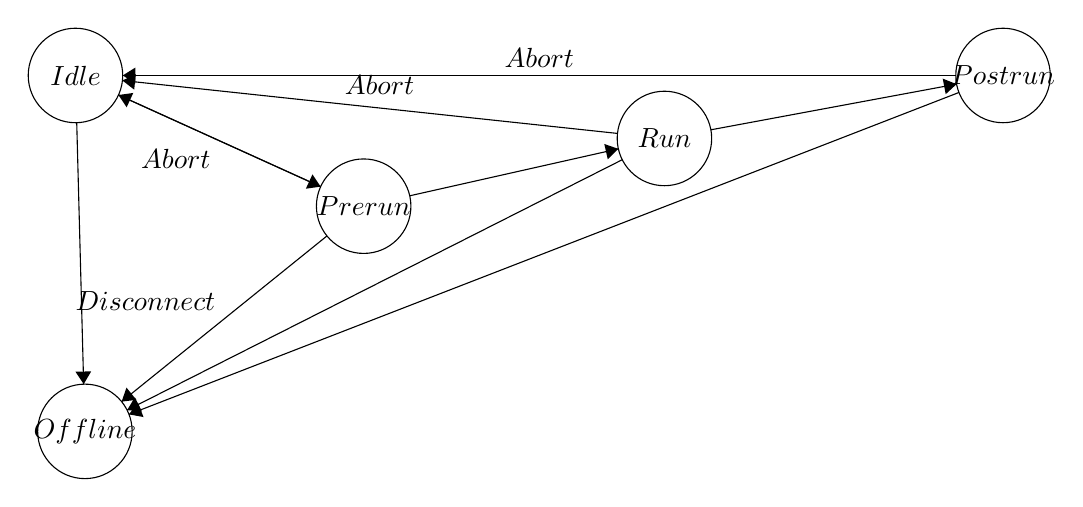
\begin{tikzpicture}[scale=0.2]
\tikzstyle{every node}+=[inner sep=0pt]
\draw [black] (11.2,-6.5) circle (3);
\draw (11.2,-6.5) node {$Idle$};
\draw [black] (29.5,-14.8) circle (3);
\draw (29.5,-14.8) node {$Prerun$};
\draw [black] (48.6,-10.5) circle (3);
\draw (48.6,-10.5) node {$Run$};
\draw [black] (70.1,-6.5) circle (3);
\draw (70.1,-6.5) node {$Postrun$};
\draw [black] (11.8,-29.1) circle (3);
\draw (11.8,-29.1) node {$Offline$};
\draw [black] (13.93,-7.74) -- (26.77,-13.56);
\fill [black] (26.77,-13.56) -- (26.25,-12.78) -- (25.83,-13.69);
\draw (17.57,-11.18) node [below] {$Abort$};
\draw [black] (32.43,-14.14) -- (45.67,-11.16);
\fill [black] (45.67,-11.16) -- (44.78,-10.85) -- (45,-11.82);
\draw [black] (51.55,-9.95) -- (67.15,-7.05);
\fill [black] (67.15,-7.05) -- (66.27,-6.7) -- (66.46,-7.69);
\draw [black] (11.28,-9.5) -- (11.72,-26.1);
\fill [black] (11.72,-26.1) -- (12.2,-25.29) -- (11.2,-25.31);
\draw [black] (27.17,-16.69) -- (14.13,-27.21);
\fill [black] (14.13,-27.21) -- (15.07,-27.1) -- (14.44,-26.32);
\draw (15.64,-21.46) node [above] {$Disconnect$};
\draw [black] (45.92,-11.85) -- (14.48,-27.75);
\fill [black] (14.48,-27.75) -- (15.42,-27.83) -- (14.97,-26.94);
\draw [black] (67.3,-7.58) -- (14.6,-28.02);
\fill [black] (14.6,-28.02) -- (15.52,-28.19) -- (15.16,-27.26);
\draw [black] (26.77,-13.56) -- (13.93,-7.74);
\fill [black] (13.93,-7.74) -- (14.45,-8.52) -- (14.87,-7.61);
\draw [black] (45.62,-10.18) -- (14.18,-6.82);
\fill [black] (14.18,-6.82) -- (14.93,-7.4) -- (15.03,-6.41);
\draw (30.5,-7.76) node [above] {$Abort$};
\draw [black] (67.1,-6.5) -- (14.2,-6.5);
\fill [black] (14.2,-6.5) -- (15,-7) -- (15,-6);
\draw (40.65,-6) node [above] {$Abort$};
\end{tikzpicture}
\caption{Possible States for the Module and their transitions}
\label{states}
\end{figure}
	\section{Instrument Service detailed command documentation}
	During the startup of the device, the clock is initialized. This is a relative timer that is being used throughout the protocol.
	\begin{verbatim*}
	var start_time = datetime.datetime.now()
	\end{verbatim*}
	
	Additionally, only the "Run" state is currently implemented in the code. The other states should behave accordingly.
	\subsection{Run initialization}

	The nomenclature differes between the OpenLab software and the instrument protocol:
\begin{center}
	\begin{tabular}{ |c|c|c| }
\hline
	\textbf{Protocol} & \textbf{OpenLab} \\
\hline\hline
	AXPRE & Prerun \\\hline
	AXINTO & Running \\\hline
	AXPOST & Postrun\\\hline
	\end{tabular}	
\end{center}

	During initialization of a run, a timetable is being sent to the instrument.
	Example wth comments added - normally each line is only terminated by \fbox{\textbackslash{}n} without further whitespaces/newlines in between:
\label{init}
\begin{lstlisting}[language=Python,escapechar=!,caption=Timetable initialisation,showspaces=true]
#TimeTable Conditional Row - AXINTO requires the command AR_START (ARST)
TTCR AXINTO, AR_START\n

#TimeTable Conditional Row - AXPOST requires the command AR_STOP (ARSP)
TTCR AXPOST, AR_STOP\n

#TimeTable Operation - For AXINTO the previous State is AXPRE
TTOP AXINTO, 0; TTSP AXPRE\n
TTOP AXINTO, 0; TTDS AXPRE\n

#TimeTable Operation - For AXPOST the previous State is AXINTO
TTOP AXPOST, 0; TTSP AXINTO\n
TTOP AXPOST, 0; TTDS AXINTO\n

#TimeTable Operation - Set AXINTO planned runtime to 180000ms (=3 minutes)
#Behave like receiving the ARSP(=Stop) command afterwards
TTOP AXINTO, !\colorbox{light-gray}{180000}!; ARSP\n

#TTOP SY(system) NO( op) - do nothing in AXPRE, disables this
TTOP AXPRE, 0; SYNO\n

#TimeTable Entry - activates the commands from before
TTEN AXPRE\n
TTEN AXINTO\n
TTEN AXPOST\n
\end{lstlisting}
When this message is received, the implementation shall take note of the highlighted value, as this is the runtime in milliseconds.
	
	\subsection{AREV}
	The \fbox{\textbf{AREV}} command is responsible for returning a Reference Time after an injection. The exact moment of setting this time depends on the instrument receiving the ARST command.
Request:
\begin{lstlisting}[language=Python,escapechar=!,caption=Request (AIC$\rightarrow{}$Instrument),showspaces=true]
AREV\n
\end{lstlisting}
Responses:
\begin{lstlisting}[language=Python,escapechar=!,caption=Response (Instrument$\rightarrow{}$AIC) - No injection yet,showspaces=true]
AREV NONE; NONE\n
\end{lstlisting}
\begin{lstlisting}[language=Python,escapechar=!,caption=Response (Instrument$\rightarrow{}$AIC) - Injection happend and run ongoing,showspaces=true]
AREV HOST, !\colorbox{light-gray}{123456}!, 223; NONE\n
\end{lstlisting}
The highlighted value (123456) is calculated as follows: 
\begin{lstlisting}[language=Python,escapechar=!,caption=calculation of injection time,breaklines=true]
# returns the measurement start time in milliseconds
injection_time = (time_of_measurement_start - start_time).total_seconds()*1000 
\end{lstlisting}
\begin{lstlisting}[language=Python,escapechar=!,caption=Response (Instrument$\rightarrow{}$AIC) - Run finished,showspaces=true]
AREV HOST, !\colorbox{light-gray}{123456}!, 223; HOST, !\colorbox{light-gray}{789123}!, 255\n
\end{lstlisting}
After a run, the end is signaled from the instrument to OpenLab / AIC by the AREV command also. In this example, the run started at 123456ms after instrument start and ran until 789123ms after instrument start (=665667ms).
So AXINTO was most likely set to be around that number.

	\subsection{ARST}
	The \fbox{\textbf{ARST}} command starts a run and sets the reference time in order to align signals in the OpenLab online view.
	\begin{verbatim}
	var time_of_measurement_start = datetime.now().millis
	var running = True
	\end{verbatim}
	\subsection{ARSP}
	The \fbox{\textbf{ARSP}} command ends a run. In regular runs this is most likely not used or only used as an internal placeholder.
	In regular runs, when the time set from the timetable elapses, the AIC requests timestamps by \fbox{\textbf{AREV}}, knows the run has ended, and officially end the run by sending additional \fbox{\textbf{ARGR}} commands.

	Else, this is the \textbf{ABORT} command to immediately stop a run.
	\subsection{AVSS}
	Requests the System Status for Channel A values.
	Since this is one of the more complex commands, multiple colors will be used in the listing and explained further down.
\begin{lstlisting}[language=Python,escapechar=!,caption=Request (AIC$\rightarrow{}$Instrument) System State Channel A,breaklines=true,showspaces=true]
AVSS\n
\end{lstlisting}
\begin{lstlisting}[language=Python,escapechar=!,caption=Response 1 (Instrument$\rightarrow{}$AIC) System State Channel A,breaklines=true,showspaces=true]
AVSS !\colorbox{VioletRed}{ON}!, !\colorbox{Melon}{0}!, 5, !\colorbox{BlueGreen}{1}!, !\colorbox{SpringGreen}{123456789}!\n
\end{lstlisting}
The \colorbox{VioletRed}{status text} can only be ON or OFF. In general this is ON, with OFF only used for a short time after a measurement.
The \colorbox{Melon}{status code} has 3 different values. When not in an active measurement, this will be \colorbox{Melon}{0}. In an active run, this value changes to \colorbox{Melon}{5}, except shortly after a run, where this changes to \colorbox{Melon}{14}.
The \colorbox{BlueGreen}{queue size} contains the number of values currently buffered on the instrument side and ready to be received. This is 0 when no values are ready to be received, otherweise greater than 0.
The \colorbox{SpringGreen}{time} returns the elapsed milliseconds since the instrument has been turned on. This value shall only increase in one session, otherwise there is an error.
	\subsection{AVDF}
The \fbox{\textbf{AVDF}} command requests the preparation of values from the queue to be requested via \fbox{\textbf{AVRD}} shortly.
\begin{lstlisting}[language=Python,escapechar=!,caption=Request (AIC$\rightarrow{}$Instrument) System State Channel A,breaklines=true,showspaces=true]
AVDF HEX, !\colorbox{BlueGreen}{3}!\n
\end{lstlisting}
Requests the preparation of 3 values. The previous AVSS command must have returned at least \colorbox{BlueGreen}{3}.
This value needs to be saved until the next AVRD command.
	\subsection{AVRD}
	Reads the prepared number of values from the instruments measurement queue.
	This should be seen in connection with the \fbox{\textbf{AVSS}} and \fbox{\textbf{AVDF}} commands.
\begin{lstlisting}[language=Python,escapechar=!,caption=Request (AIC$\rightarrow{}$Instrument) Read Values from Queue,breaklines=true,showspaces=true]
AVRD\n
\end{lstlisting}
\begin{lstlisting}[language=Python,escapechar=!,caption=Response (Instrument$\rightarrow{}$AIC) Read Values from Queue,breaklines=true,showspaces=true]
AVRD HEX, !\colorbox{BlueGreen}{002}!;!\colorbox{light-gray}{0023F73C}!0023F725\n
\end{lstlisting}



	\subsection{ARSS}
	The \fbox{\textbf{ARSS}} command requests the channel A RUN SYSTEM STATE.

\begin{lstlisting}[language=Python,escapechar=!,caption=Request (AIC$\rightarrow{}$Instrument) Read Values from Queue,breaklines=true,showspaces=true]
ARSS\n
\end{lstlisting}
\begin{lstlisting}[language=Python,escapechar=!,caption=Response (Instrument$\rightarrow{}$AIC) Read Values from Queue,breaklines=true,showspaces=true]
ARSS !\colorbox{BlueGreen}{statustext}!, !\colorbox{light-gray}{statuscode}!\n
\end{lstlisting}
The \colorbox{BlueGreen}{statustext} is either READY in regular online mode, RUN during a measurement or NOT\textunderscore{}READY shortly after a measurement until a \fbox{\textbf{ARGR}} command is received.
The \colorbox{light-gray}{statuscode} in these cases is 0 for READY, 5 for RUN and 14 for NOT\textunderscore{}READY.
These status values are not user-facing and only for internal handling of state.

	\subsection{AVSL}
	Requests or sets the value sampling rate
\begin{lstlisting}[language=Python,escapechar=!,caption=Requesting (AIC$\rightarrow{}$Instrument) Sampling rate currently set,breaklines=true,showspaces=true]
AVSL ?\n
\end{lstlisting}
\begin{lstlisting}[language=Python,escapechar=!,caption=Response (Instrument$\rightarrow{}$AIC) Sampling rate currently set,breaklines=true,showspaces=true]
AVSL !\colorbox{light-gray}{1000}!\n
\end{lstlisting}
The value 1000 in this case means once per second (1Hz).
\begin{lstlisting}[language=Python,escapechar=!,caption=Setting (AIC$\rightarrow{}$Instrument) Sampling rate ,breaklines=true,showspaces=true]
AVSL 1000\n
\end{lstlisting}
\begin{lstlisting}[language=Python,escapechar=!,caption=Response to setting Sampling Rate (Instrument$\rightarrow{}$AIC) ,breaklines=true,showspaces=true]
AVSL 1000\n
\end{lstlisting}
For a sampling rate of 10Hz, the value will be 100 etc.
	\subsection{ARGR}
	The \fbox{\textbf{ARGR}} command is being sent shortly before an injection is happening and can be seen as a "GET READY" method.
	There is no expected answer from the Instrument to the AIC to this command.

	\subsection{ATRD}
	The \fbox{\textbf{ATRD}} command is a basic PING/PONG mechanic.
\begin{lstlisting}[language=Python,escapechar=!,caption=Request (AIC$\rightarrow{}$Instrument),breaklines=true,showspaces=true]
ATRD\n
\end{lstlisting}
\begin{lstlisting}[language=Python,escapechar=!,caption=Response (Instrument$\rightarrow{}$AIC) ,breaklines=true,showspaces=true]
ATRD 255\n
\end{lstlisting}

	\subsection{ARBM}
	The \fbox{\textbf{ARBM}} command requests configures the button mode for channel A.
\begin{lstlisting}[language=Python,escapechar=!,caption=Request (AIC$\rightarrow{}$Instrument),breaklines=true,showspaces=true]
ARBM ?\n
\end{lstlisting}
\begin{lstlisting}[language=Python,escapechar=!,caption=Response (Instrument$\rightarrow{}$AIC) ,breaklines=true,showspaces=true]
ARBM OFF, OFF\n
\end{lstlisting}

Setting the button mode works accordingly
\begin{lstlisting}[language=Python,escapechar=!,caption=Request (AIC$\rightarrow{}$Instrument),breaklines=true,showspaces=true]
ARBM OFF, OFF\n
\end{lstlisting}
\begin{lstlisting}[language=Python,escapechar=!,caption=Response (Instrument$\rightarrow{}$AIC) ,breaklines=true,showspaces=true]
ARBM OFF, OFF\n
\end{lstlisting}

	\subsection{TTSS}
	The \fbox{\textbf{TTSS}} command requests the timetable system status
\begin{lstlisting}[language=Python,escapechar=!,caption=Request (AIC$\rightarrow{}$Instrument),breaklines=true,showspaces=true]
TTSS !\colorbox{light-gray}{state}!\n
\end{lstlisting}
The \colorbox{Orange}{state} here is either AXPRE, AXINTO or AXPOST as defined above.
\begin{lstlisting}[language=Python,escapechar=!,caption=Response (Instrument$\rightarrow{}$AIC) ,breaklines=true,showspaces=true]
TTSS state, !\colorbox{Lavender}{current-status}!, !\colorbox{Purple}{currenttime}!, !\colorbox{YellowGreen}{plannedtime}!\n
\end{lstlisting}
The \colorbox{Lavender}{current-status} is either ENABLED if this state should be running after ARST, DISABLED if this state should be skipped, or RUNNING if this is the currently active state.
The \colorbox{Purple}{currenttime} is milliseconds since Start of the RUN (not instrument!).
The \colorbox{YellowGreen}{plannedtime} is what gets set in the init phase (see \ref{init}).

In our implementation, only the Prerun and Run state are actively used.

If no run is active, the response to a request will alsways be 
\begin{lstlisting}[language=Python,escapechar=!,caption=Response (Instrument$\rightarrow{}$AIC) ,breaklines=true,showspaces=true]
TTSS state, !\colorbox{Lavender}{current-status}!, DISABLED, -1, 0\n
\end{lstlisting}

Additionally, if this is our internal trigger to set a RUN\textbackslash{}STOPTIME and set the \fbox{\textbf{ARSS}} state to NOT\textbackslash{}READY until \fbox{\textbf{ARGR}} is received again.
By setting RUN\textbackslash{}STOPTIME, the next \fbox{\textbf{AREV}} request will return that the run ended.

NOTE: In our implementation, we keep the RUNNING state until ARGR is received.
	\subsection{SYSN}
	The \fbox{\textbf{SYSN}} command returns the system Serial Number
\begin{lstlisting}[language=Python,escapechar=!,caption=Request (AIC$\rightarrow{}$Instrument),breaklines=true,showspaces=true]
SYSN\n
\end{lstlisting}
\begin{lstlisting}[language=Python,escapechar=!,caption=Response (Instrument$\rightarrow{}$AIC) ,breaklines=true,showspaces=true]
SYSN LIFERADIO1\n
\end{lstlisting}


	\subsection{SYID}
	The \fbox{\textbf{SYID}} command returns the system ID and Firmware.
\begin{lstlisting}[language=Python,escapechar=!,caption=Request (AIC$\rightarrow{}$Instrument),breaklines=true,showspaces=true]
SYID\n
\end{lstlisting}
\begin{lstlisting}[language=Python,escapechar=!,caption=Response (Instrument$\rightarrow{}$AIC) ,breaklines=true,showspaces=true]
SYID HP35900E, Rev E.02.04.32\n
\end{lstlisting}
\end{document}